\chapter{Composite}
\section{Intento}

Comporre oggetti in strutture ad albero per rappresentare gerarchie parziali. Il Composite consente ai clienti di trattare i singoli oggetti e le composizioni di oggetti in modo uniforme.


%---
\section{Prestruttura}

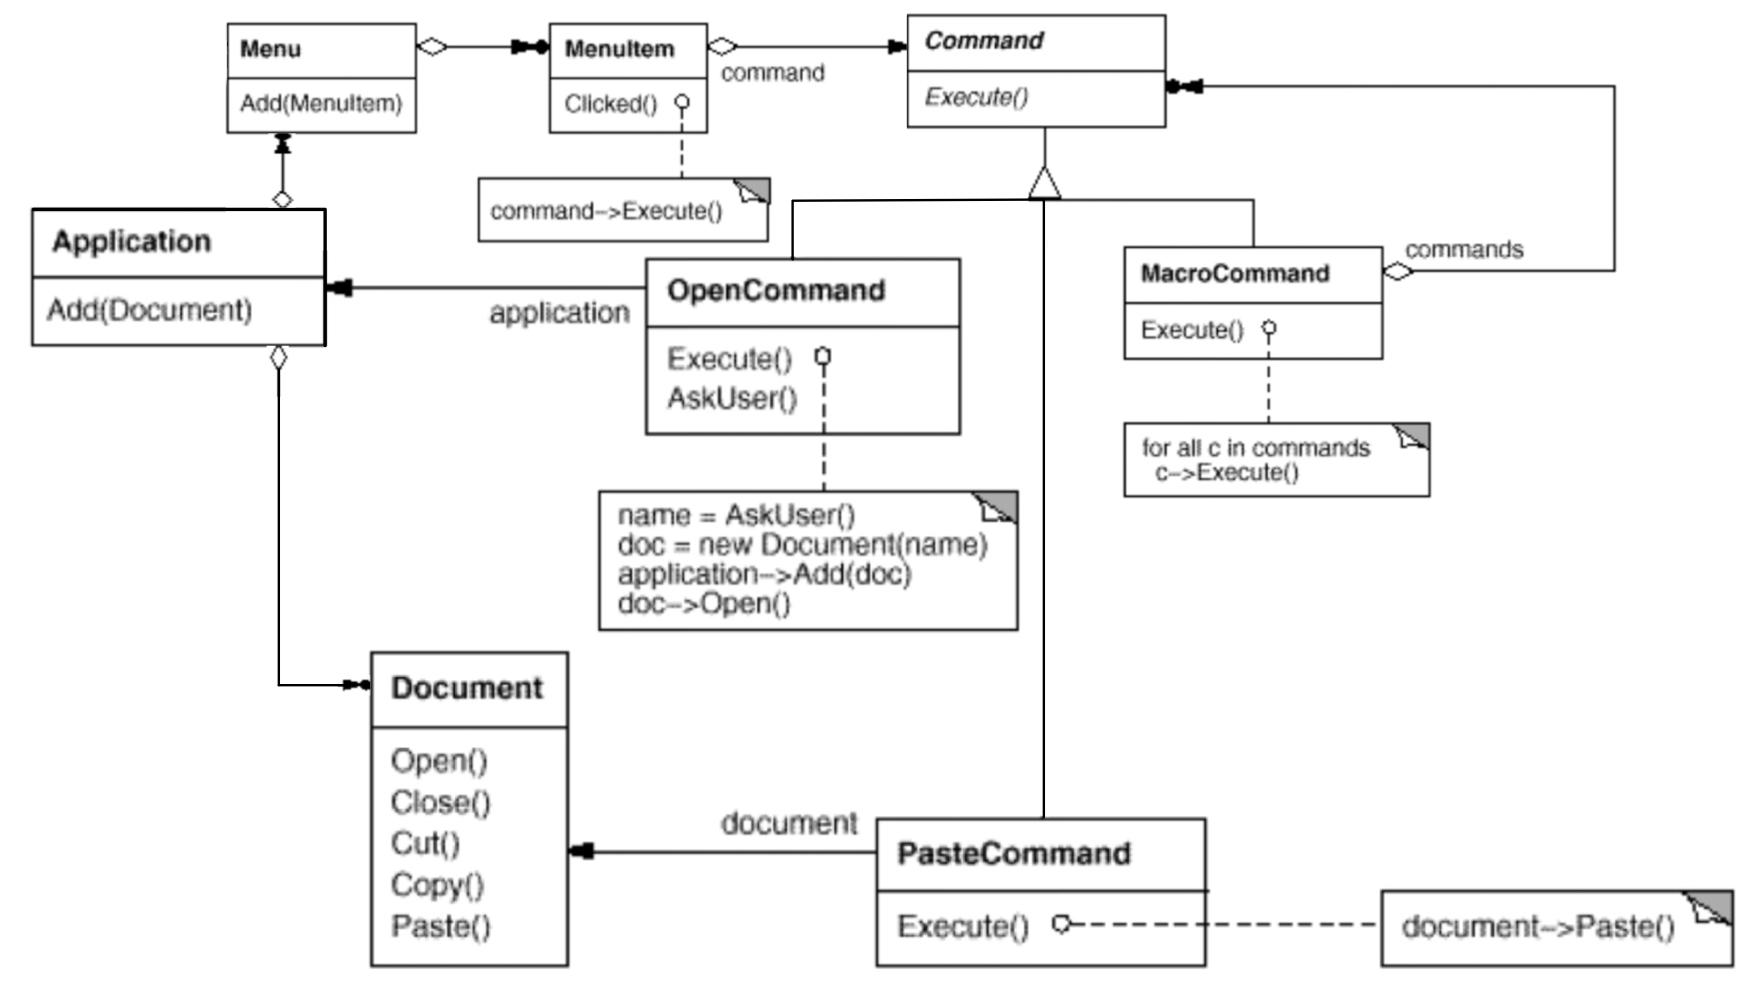
\includegraphics[width=\textwidth]{/Users/matt/Documents/LaTex/Design Pattern LaTex/Composite/Prestructure1}


%---
\section{Struttura}

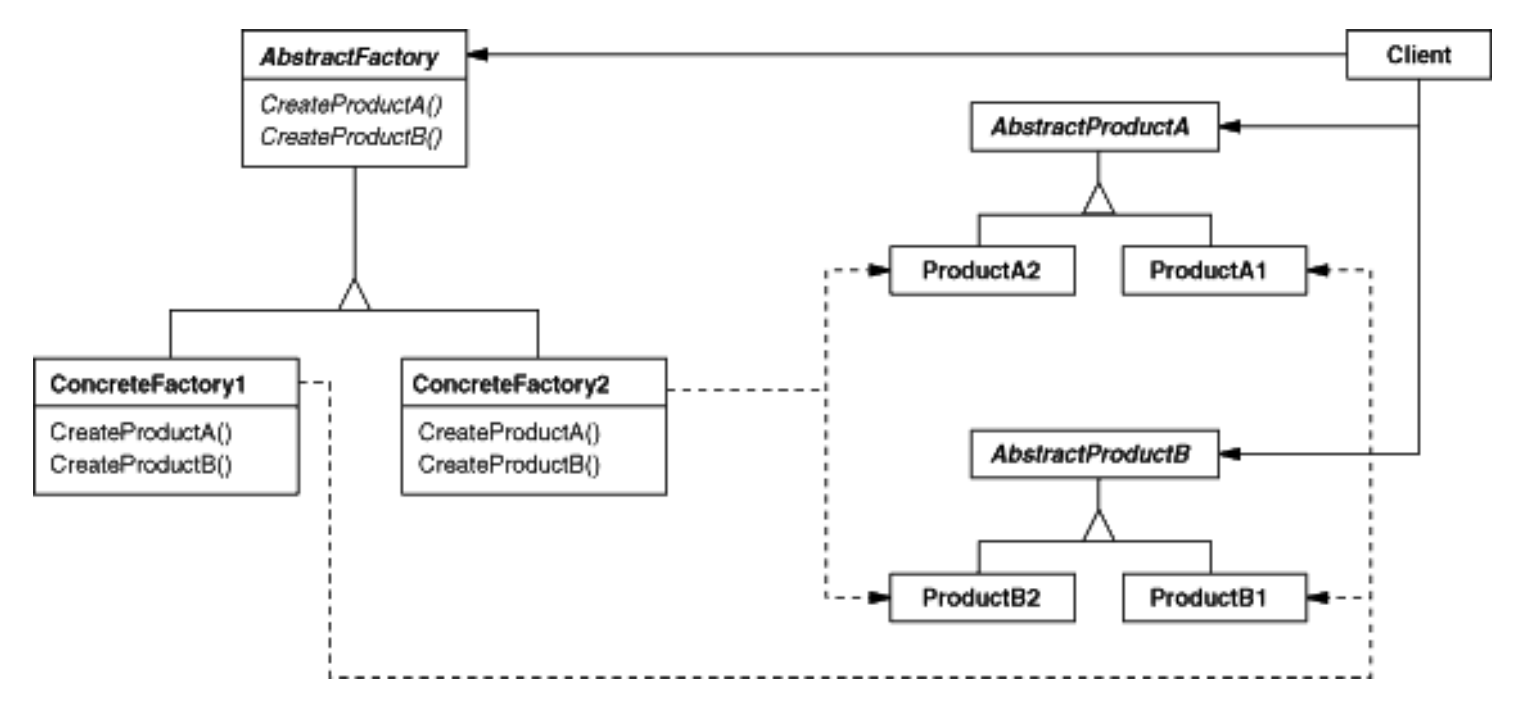
\includegraphics[width=\textwidth]{/Users/matt/Documents/LaTex/Design Pattern LaTex/Composite/Structure1}


%---
\section{Implementazione}

\subsection{Condivisione di Component.}
È spesso utile condividere i Component, ad esempio, per ridurre i requisiti di archiviazione. Ma quando un componente non può avere più di un genitore, la condivisione di Component diventa difficile.

Una possibile soluzione è che i figli memorizzino più genitori. (Il modello Flyweight (218) mostra come rielaborare un design per evitare di memorizzare i genitori del tutto)

\subsection{Massimizzare l'interfaccia del componente.}
Uno degli obiettivi del pattern Composite è rendere i clienti ignari delle classi che stanno utilizzando.

Per raggiungere questo obiettivo, la classe Component definisce le operazioni più comuni, fornendo quindi implementazioni predefinite per le sottoclassi Leaf e Composite, che le sovrascriveranno.

In che modo Component può fornire un'implementazione predefinita a Leaf? Le classi Leaf possono utilizzare l'implementazione predefinita, ma le classi composite la reimplementeranno per restituire i propri figli.

\subsection{Dichiarazione delle operazioni di gestione del figlio.}
Meglio dichiarare le operazioni Aggiungi e Rimuovi nel Component e renderle significative per le classi Leaf, o dichiararle e definirle solo in Composite e nelle sue sottoclassi?

La decisione prevede un compromesso tra sicurezza e trasparenza:

\begin{enumerate}
    \item La definizione alla radice della gerarchia offre trasparenza, poiché si trattano i Component in modo uniforme. Ne viene meno la sicurezza, dato che i clienti possono provare ad aggiungere e rimuovere oggetti dalle Leaf.

    L'unico modo per fornire trasparenza è definire le operazioni di aggiunta e rimozione predefinite in Component. 

    Questo crea un problema: non c'è modo di implementare Add di Component senza introdurre la possibilità che fallisca o che permetta un tentativo di aggiungere qualcosa a una Leaf creando un bug.

    Di solito è meglio far fallire Aggiungi e Rimuovi per impostazione predefinita (magari sollevando un'eccezione) se il Component non può avere figli o se l'argomento di Rimuovi non è figlio di Component.

    \item Definire la gestione dei figli nella classe Composite ti dà sicurezza, perché qualsiasi tentativo di aggiungere o rimuovere oggetti dalle Leaf verrà catturato. Se perdi in trasparenza, perché Leaf e Composite hanno interfacce diverse.

    Se opti per la sicurezza, a volte potresti perdere le informazioni sul tipo e dover convertire un Componente in un Composite.
\end{enumerate}

Senza ricorrere a un cast non sicuro per i tipi possiamo dichiarare un'operazione nella classe Component:

\begin{itemize}
    \item in Componente:
    
    \begin{lstlisting}[language=java]
        Composite GetComposite() {
            return 0;
        }
    \end{lstlisting}

    \item in Composite:
    
    \begin{lstlisting}[language=java]
        Composite GetComposite() {
            return this;
        }
    \end{lstlisting}

\end{itemize}

GetComposite ti consente di interrogare un componente per vedere se è un composto.

\begin{lstlisting}[language=java]
    Composite aComposite = new Composite();
    Leaf aLeaf = new Leaf();

    Component aComponent;
    Composite test;
    
    aComponent = aComposite;
    if (test = aComponent.GetComposite()) {
        test.Add(new Leaf);
    }

    aComponent = aLeaf;
    if (test = aComponent.GetComposite()) {
        test.Add(new Leaf); // not add leaf
    }
\end{lstlisting}

\subsection{Il Component dovrebbe implementare un elenco di Component?}
Definire l'insieme dei figli come una variabile di istanza nella classe Component comporta una penalità di spazio per ogni Leaf (solo se nella struttura ci sono pochi figli).

\subsection{Memorizzazione nella cache per migliorare le prestazioni.}
Il Composit può memorizzare nella cache i risultati effettivi o solo le informazioni che gli consentono di cortocircuitare l'attraversamento o la ricerca. 

Se stai usando la memorizzazione nella cache, devi definire un'interfaccia per dire ai Composite che le loro cache non sono valide dato che si potrebbe usare un Draw quando un figlio non è visibile, non avendo quindi nessun apparente modifica.

\subsection{Chi dovrebbe eliminare i Component?}
Nelle lingue senza raccolta di rifiuti, di solito è meglio rendere un Composit responsabile dell'eliminazione dei suoi figli quando viene distrutto.

Un'eccezione è quando gli oggetti Leaf sono immutabili e quindi possono essere condivisi.


%---
\section{Esempio Java}
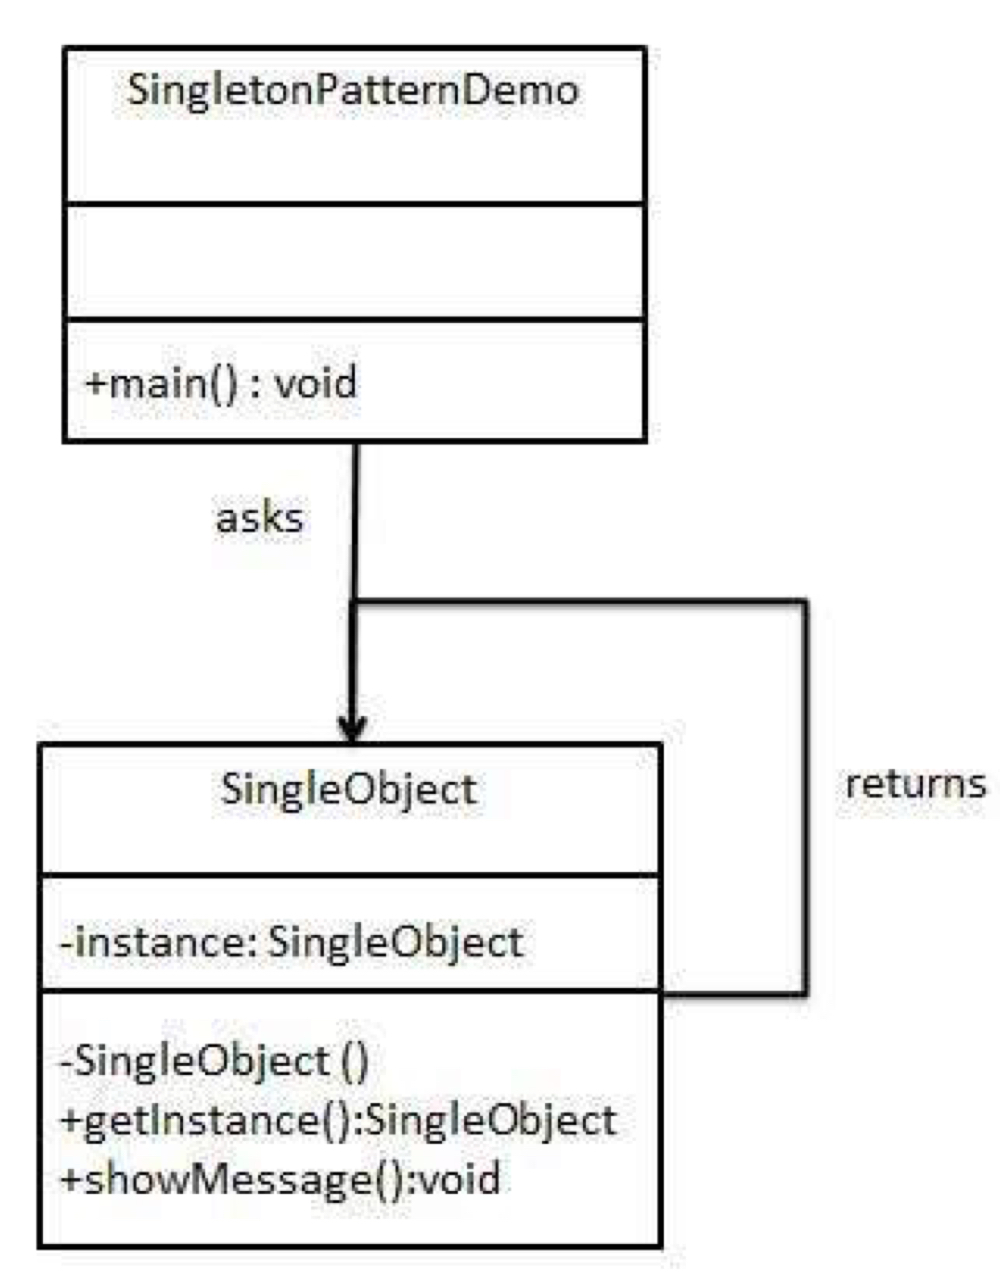
\includegraphics[width=7cm]{/Users/matt/Documents/LaTex/Design Pattern LaTex/Composite/Example1}

\subsection{Employee.java}
\begin{lstlisting}[language=java]
    public class Employee {
        private String name;
        private String dept;
        private int salary;
        private List<Employee> subordinates; // Design pattern Composite
    
        public Employee(String name, String dept, int salary){
            this.name = name;
            this.dept = dept;
            this.salary = salary;
            this.subordinates = new ArrayList<Employee>();
        }
    
        public void addSubordinates(Employee employee){
            subordinates.add(employee);
        }
    
        public void removeSubordinates(Employee employee){
            subordinates.remove(employee);
        }
    
        public List<Employee> getSubordinates(){
            return subordinates;
        }
    
        @Override
        public String toString(){
            return ("Composite.Employee : [ Name: " + name +
                                         ", dept: " + dept +
                                       ", salary: " + salary + " ]");
        }
    }
\end{lstlisting}

\subsection{main}
\begin{lstlisting}[language=java]
    public class CompositePatternDemo {
        public static void main(String[] args) {
            Employee ceo = new Employee("Adriana", "Main", 30000);
    
            Employee headMark = new Employee("Roberto", "Marketing", 20000);
            Employee clerk1 = new Employee("Laura", "Marketing", 10000);
            Employee clerk2 = new Employee("Alessandro", "Marketing", 10000);
    
            Employee headDev = new Employee("Luigi", "Development", 20000);
            Employee dev1 = new Employee("Ilaria", "Development", 10000);
            Employee dev2 = new Employee("Giovanni", "Development", 10000);
    
            ceo.addSubordinates(headMark);
            ceo.addSubordinates(headDev);
    
            headMark.addSubordinates(clerk1);
            headMark.addSubordinates(clerk2);
    
            headDev.addSubordinates(dev1);
            headDev.addSubordinates(dev2);
    
            System.out.println(ceo);
    
            List<Employee> ceoSubordinates = ceo.getSubordinates();
            Iterator<Employee> ceoSubIter = ceoSubordinates.iterator();
    
            while (ceoSubIter.hasNext()) {
                Employee e = ceoSubIter.next();
                System.out.println(e);
    
                List<Employee> headSubordinates = e.getSubordinates();
                Iterator<Employee> headSubIter = headSubordinates.iterator();
                
                while (headSubIter.hasNext()) {
                    System.out.println(headSubIter.next());
                }
            }
        }
    }
\end{lstlisting}